\section{引言}
人类依靠集体智慧与协作能力处理复杂的长程工作~\cite{gao2025evolvesurvey,DBLP:journals/corr/abs-2510-23587,DBLP:journals/corr/abs-2510-17586}。如今，智能体也在不断迈向类似的复杂多轮任务~\cite{yao2024tau, zhang2025autoenv, xu2026unlocking}，因此，设计良好的智能体系统已成为突破单一模型性能上限的重要途径~\cite{liu2025advances}。

\begin{figure}[t!]
    \centering
    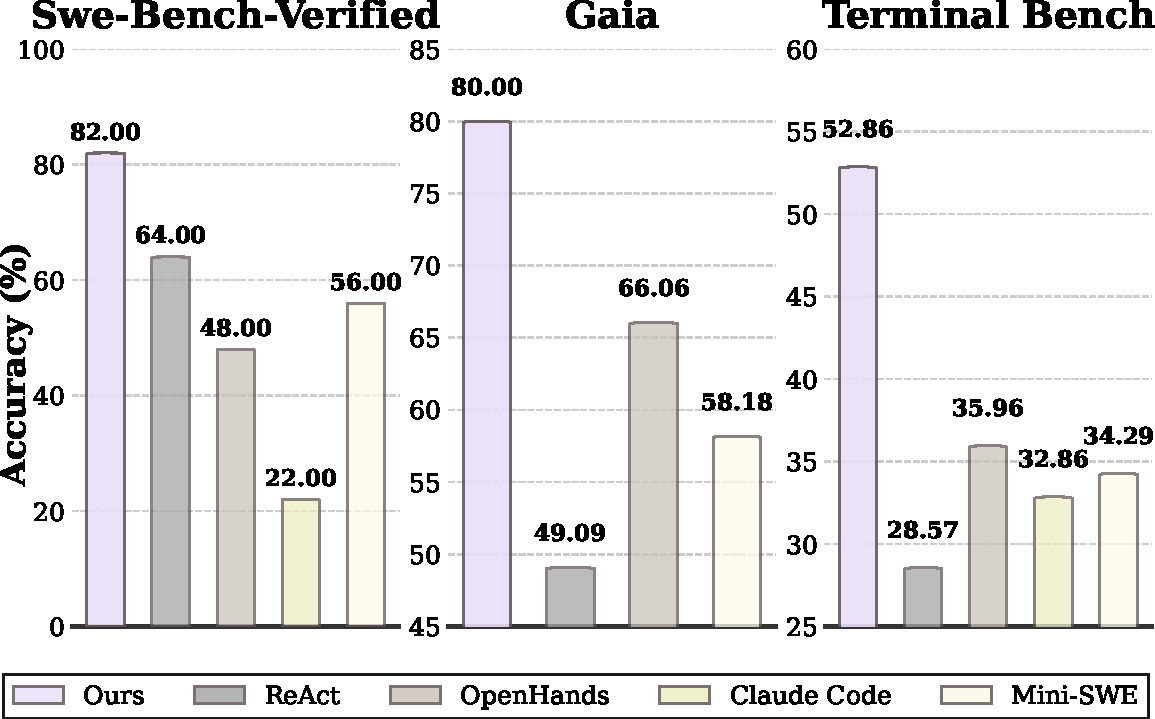
\includegraphics[width=\linewidth]{figures/abs.pdf}
    \caption{在 Gemini-3-Flash 配置下，\our 与其他常用智能体框架在三个高难度智能体基准（GAIA、Terminal-Bench 2.0 和 SWE-Bench-Verified）上的整体性能对比。}
    \label{fig:performance}
\end{figure}

为应对日益复杂的应用场景，早期工作通常依赖固定的协作流程或多智能体系统~\cite{hong2023metagpt, hu2025owl, DBLP:journals/corr/abs-2510-17586}。多智能体协作虽然有助于任务分解，但在开放式环境中往往带来显著的协调开销，且难以精细控制上下文路由，容易出现含噪信息过度共享或关键信息被遗漏的问题，从而使稳健的长程执行变得困难~\cite{gao2025single}。

\begin{figure*}[htbp]
    \centering
    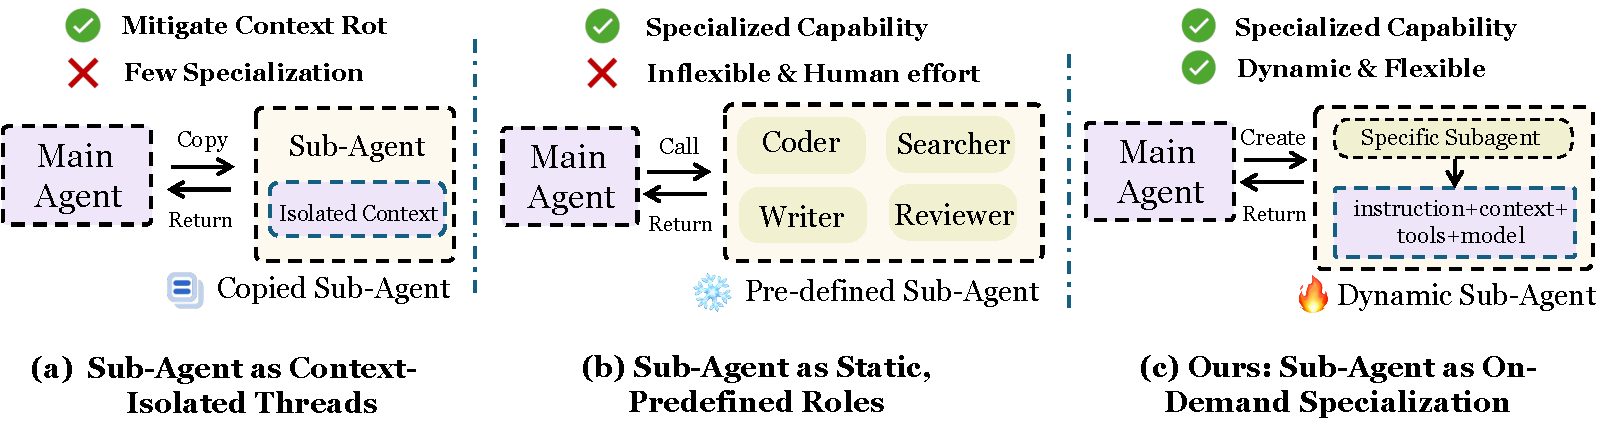
\includegraphics[width=\linewidth]{figures/diff.pdf}
    \caption{“子智能体即工具”方法对比。\textbf{(a) 将子智能体视为上下文隔离线程}可以缓解上下文退化，却无法按需专门化。\textbf{(b) 将子智能体视为静态角色}能够提供专用能力，但缺乏灵活性，存在能力覆盖空缺，并需要大量人工工程。\textbf{(c) 我们的按需专门化子智能体}通过实例化统一四元组抽象 \textsc{(Instruction, Context, Tools, Model)}，即时创建针对具体任务定制的执行器。}
    \label{fig:diff}
\end{figure*}

因此，较新的方法逐渐转向更实用的“子智能体即工具”范式：主智能体（即编排器）通过显式工具调用，将任务委派给子智能体。然而，现有设计在实践中仍缺乏灵活性，并经常退化为图~\ref{fig:diff} 所示的两种受限模式：
(1) \textit{将子智能体视为上下文隔离线程。}THREAD~\cite{schroeder2025thread} 和 Context-Folding~\cite{sun2025scaling} 等系统主要把子智能体视为彼此隔离的上下文线程，以避免上下文退化~\citep{hong2025context}。但现实任务中的子任务往往需要专门能力，因此这类系统无法充分发挥专用子智能体的潜力。
(2) \textit{将子智能体视为静态角色。}Claude Code~\cite{anthropic_claude_code_subagents} 和 Chain-of-Agents~\cite{li2025chain} 等系统将每个子智能体设定为静态角色，其能力与协作模式通常被硬编码。预先定义的一组子智能体无法覆盖开放环境中动态出现的各类子任务，而且高度依赖人工工程，难以适配不同环境。

本文提出 \our{}，一个面向复杂长程任务的智能体框架。我们的核心观点是从\textbf{按需专门化}的角度看待子智能体，如图~\ref{fig:diff}(c) 所示。我们认为，子智能体应被视为灵活的抽象单元，而不是预定义的固定角色。系统由此可以在运行时动态组合能力，根据具体任务需要实例化定制的子智能体。
具体而言，\emph{任意}智能体都可以通过统一四元组 \textsc{(instruction, context, tools, model)} 描述为可实例化单元。专门化围绕智能体求解任务所需的两个互补维度展开：(1) \emph{工作记忆（instruction, context）}，即智能体必须达成的目标，以及作出判断时应依据的证据。尤其是，context 属性只注入与当前子任务最相关的信息，从而过滤可能造成干扰的细节。(2) \emph{能力（tools, model）}，即为达成目标，智能体被赋予哪些可执行能力。系统按子任务组合特定工具与模型，使每个子智能体都具备精确且任务专用的功能。二者共同使系统能够为每项任务自动创建专用子智能体。

基于这一按需专门化视角，我们进一步引入专用编排器。它直接操作四元组接口，动态自动创建定制子智能体。编排器本身不执行任务，只负责系统编排：将总体目标动态分解为下一项子任务，通过显式工具调用创建专门化的定制子智能体，并将执行工作委派给它。
这种解耦设计具有多项优势。第一，动态创建机制可以让每个子智能体拥有独特能力和干净的工作上下文，显著提高任务执行准确率。第二，编排器不依赖子智能体的内部实现，因此子智能体可以完全即插即用。第三，编排器可以从交互经验中训练或学习，其能力范围既包括创建智能体的基础技能，也包括自适应模型选择等高级特性，从而在成本与性能之间取得更优平衡。

大量实验表明，\our{} 在开放世界环境中具有更强的性能和更广泛的泛化能力。我们首先在免训练设置下，对三个高难度智能体基准进行评测：Terminal-Bench 2.0~\cite{tbench_2025}（Bash 环境）、SWE-Bench~\cite{jimenez2023swe}（编程环境）和 GAIA~\cite{mialon2023gaia}（数字世界环境）。如图~\ref{fig:performance} 所示，我们的方法在所有基准上均持续优于具有代表性的子智能体编排方法~\cite{anthropic_claude_code_subagents}和广泛使用的智能体框架~\cite{wang2024openhands, yang2024sweagent}。尤其是在搭配 \texttt{Gemini3-Flash} 时，我们的框架取得了 $16.28\%$ 的提升，验证了该编排模型在复杂长程任务中的优越性。

更重要的是，\our 自然支持从经验中学习编排策略。我们通过两种方式实例化这一能力：(1) 使用监督微调提升编排器的子任务分解与四元组合成能力，使 GAIA 上的编排质量提升 $11.51\%$ pass@1；(2) 使用上下文学习优化成本感知路由，使 GAIA pass@1 提升 $3.03\%$，同时将平均成本降低 $18.5\%$，得到更优的成本与性能帕累托前沿。

总体而言，我们的贡献如下：
\begin{itemize}
    \item 我们提出 \our，一个以编排器为中心的智能体系统。它通过统一四元组接口 \textsc{(Instruction, Context, Tools, Model)}，将子智能体视为可\emph{动态创建}的执行器，从而以任务充分的上下文和显式能力控制实现按需专门化。
    \item \our 在 Terminal-Bench 2.0、SWE-Bench-Verified 和 GAIA 上取得了强劲的免训练性能，并持续优于常用智能体系统。与 Gemini-3-Flash 搭配时，相比最强基线取得了 $16.28\%$ 的相对提升。
    \item 我们从两个互补角度表明该设计下的编排策略是可学习的：监督微调可以提升基础任务编排能力（$+11.51\%$），通过上下文学习实现的成本感知路由则带来更优的成本与性能帕累托权衡（平均成本降低 $18.5\%$）。
\end{itemize}
